% Created 2022-11-16 mer 14:32
% Intended LaTeX compiler: pdflatex
\documentclass[presentation]{beamer}
\usepackage[utf8]{inputenc}
\usepackage[T1]{fontenc}
\usepackage{graphicx}
\usepackage{longtable}
\usepackage{wrapfig}
\usepackage{rotating}
\usepackage[normalem]{ulem}
\usepackage{amsmath}
\usepackage{amssymb}
\usepackage{capt-of}
\usepackage{hyperref}
\usepackage{minted}
\usepackage[, french]{babel}
\usepackage{svg}
\logo{
\includegraphics[width=.1\textwidth]{../../by-sa.png}}
\usetheme{metropolis}
\usecolortheme{}
\usefonttheme{}
\useinnertheme{}
\useoutertheme{}
\author{Guy Bégin}
\date{\today}
\title{Circuits logiques combinatoires et séquentiels}

\hypersetup{
 pdfauthor={Guy Bégin},
 pdftitle={Circuits logiques combinatoires et séquentiels},
 pdfkeywords={},
 pdfsubject={},
 pdfcreator={Emacs 28.1 (Org mode 9.5.4)}, 
 pdflang={French}}
\begin{document}

\maketitle

\section{Logique programmable}
\label{sec:orgfbb2c51}
\begin{frame}[label={sec:org2a6c997}]{Objectifs}
\begin{itemize}
\item Être familier avec les différents types de composants logiques programmables
\item Pouvoir identifier les avantages et limitations des différents types
\item Comprendre le fonctionnement d'une matrice logique programmable
\item Comprendre le fonctionnement d'un composant logique à matrice programmable
\item Comprendre le fonctionnement d'un circuit séquentiel programmable
\item Être familier avec le concept de bloc logique programmable
\item Comprendre l'organisation d'une cellule logique programmable et
apprécier sa flexibilité
\end{itemize}
\end{frame}

\begin{frame}[label={sec:orge15a8ba}]{Dispositifs programmables}
\begin{itemize}
\item On a vu qu'une mémoire ROM est un dispositif logique programmable qui, grâce à la matrice d'interconnexion entre son décodeur (qui génère tous les minterms) et les portes OU de sortie, permet de réaliser des fonctions logiques arbitraires.

\item D'autres composants utilisent à divers degrés cette approche pour offrir des possibilités de configuration flexibles.

\item Il existe une grande variété de dispositifs programmables, des plus simples aux plus complexes.

\item De nombreux manufacturiers offrent des variantes plus ou moins équivalentes dans chacune des gammes de produits.

\item Nous allons nous limiter à présenter brièvement les grandes familles typiques, en ordre de complexité croissante.
\end{itemize}
\end{frame}

\begin{frame}[label={sec:org3d1e205}]{Matrice logique programmable (PLA)}
\begin{itemize}
\item Une \alert{matrice logique programmable} (en anglais, \emph{Programmable Logic Array}, (PLA)) est un dispositif spécifiquement conçu pour la réalisation de fonctions combinatoires arbitraires.

\item Elle fonctionne selon une approche qui s'apparente à l'utilisation d'une mémoire morte pour réaliser une fonction logique arbitraire.

\item La figure \ref{fig:org88f1f45} montre une matrice permettant de réaliser deux fonctions pouvant comporter jusqu'à quatre termes produits de trois variables.
\end{itemize}
\end{frame}

\begin{frame}[label={sec:org0c34b95}]{Matrice logique programmable}
\begin{figure}[htbp]
\centering
\includesvg[scale=0.55]{../../Sources_images_logiques/images/pla}
\caption{\label{fig:org88f1f45}Matrice logique programmable}
\end{figure}
\end{frame}

\begin{frame}[label={sec:org7207d6a}]{Matrice logique programmable (PLA) \ldots{} 2}
\begin{itemize}
\item Puisque le nombre de termes produits est limité, il n'est généralement pas possible de se baser directement sur les minterms des fonctions pour l'implémentation.

\item On doit donc simplifier les fonctions avant l'implémentation.

\item Un même terme produit peut contribuer à plus d'une fonction.

\item La programmation des portes XOR de sortie permet de choisir la fonction directe ou son complément.

\item Les PLAs offerts sur le marché proposent des configurations avec des plus grands nombres d'entrées, de termes et de sorties, typiquement des dizaines.
\end{itemize}
\end{frame}

\begin{frame}[label={sec:org0671f17}]{Logique à matrice programmable (PAL)}
\begin{itemize}
\item Les dispositifs à \alert{logique à matrice programmable} (an anglais, \emph{Programmable Array Logic} (PAL)) sont une autre variante sur ce thème, avec une matrice OU fixe et une matrice ET configurable.

\item Ils sont moins flexibles que les PLAs.

\item La figure \ref{fig:orgfae8149} montre un dispositif de logique à matrice programmable à quatre variables d'entrée, permettant de réaliser trois fonctions pouvant comporter jusqu'à trois minterms.
\end{itemize}
\end{frame}

\begin{frame}[label={sec:orgcb40d17}]{Logique à matrice programmable}
\begin{figure}[htbp]
\centering
\includesvg[scale=0.375]{../../Sources_images_logiques/images/pal}
\caption{\label{fig:orgfae8149}Logique à matrice programmable}
\end{figure}
\end{frame}

\begin{frame}[label={sec:orgc99058f}]{Logique à matrice programmable (PAL) \ldots{} 2}
\begin{itemize}
\item Les sorties (directes et complémentée pour la première fonction) peuvent être acheminées aux entrées des autres fonctions.

\item Encore ici, le nombre de termes produits est limité, et on doit simplifier les fonctions avant l'implémentation.

\item Cependant, puisqu'il n'y a pas de matrice OU, il n'est pas possible de partager un terme produit entre deux fonctions.

\item Les PALs offerts sur le marché proposent des configurations avec des plus grands nombres d'entrées d'entrées, de termes et de sorties, typiquement des dizaines.
\end{itemize}
\end{frame}

\begin{frame}[label={sec:org1415c3e}]{Logique programmable séquentielle}
\begin{itemize}
\item En combinant un dispositif logique programmable (en anglais, \emph{Programmable Logic Device}, (PLD)) avec un certain nombre de bascules, il est possible de proposer un circuit programmable séquentiel.

\item La configuration générale est telle qu'illustré sur la figure \ref{fig:org7be87bf}.
\end{itemize}
\end{frame}

\begin{frame}[label={sec:orgd709b0e}]{Modèle de circuit séquentiel programmable}
\begin{figure}[htbp]
\centering
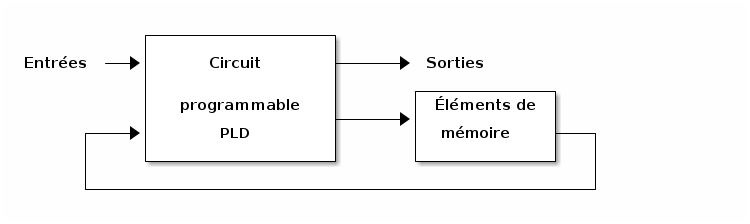
\includegraphics[scale=0.55]{../../Sources_images_logiques/images/circuit_seq_prog.png}
\caption{\label{fig:org7be87bf}Modèle de circuit séquentiel programmable}
\end{figure} 
\end{frame}

\begin{frame}[label={sec:org167b53c}]{Dispositifs programmables complexes}
\begin{itemize}
\item Plusieurs fabricants proposent une variété de dispositifs de ce type, avec diverses options de configuration, d'interconnexion, etc.

\item On offre par exemple des dispositifs complexes qui combinent plusieurs cellules programmables sur un même circuit intégré, reliables au moyen d'un réseau d'interconnexion configurable.

\item La disposition générale de ce genre de dispositif complexe est présentée à la figure \ref{fig:org7272ed0}.
\end{itemize}
\end{frame}

\begin{frame}[label={sec:orgc056e63}]{Modèle de circuit séquentiel programmable complexe}
\begin{figure}[htbp]
\centering
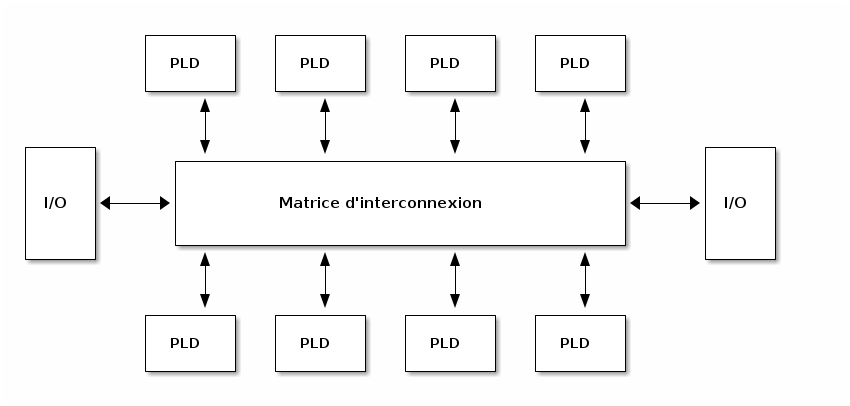
\includegraphics[scale=0.375]{../../Sources_images_logiques/images/CPLD.png}
\caption{\label{fig:org7272ed0}Modèle de circuit séquentiel programmable complexe}
\end{figure}
\end{frame}

\begin{frame}[label={sec:org4dec980}]{Circuits intégrés programmables}
\begin{itemize}
\item La version la plus sophistiquée des circuits logiques programmables est sans contredit le circuit intégré programmable (en anglais, \emph{Field Programmable gate array}, (FPGA)).

\item Un FPGA est constitué d'une matrice de blocs polyvalents appelés \alert{blocs logiques programmables} qui permettent, selon leur configuration, de réaliser n'importe quelle fonction logique.

\item Un bloc logique est typiquement constitué d'une ou de quelques \alert{cellules logiques} élémentaires.
\end{itemize}
\end{frame}

\begin{frame}[label={sec:orgb4b357d}]{Cellule logique}
La figure \ref{fig:orgabd025e} montre une version simplifiée d'une cellule logique comportant:
\begin{itemize}
\item un tableau de correspondance (LUT) à quatre entrées
\item un additionneur complet
\item une cellule de mémoire
\end{itemize}
\end{frame}

\begin{frame}[label={sec:orgd509ea5}]{Cellule logique}
\begin{figure}[htbp]
\centering
\includesvg[scale=0.75]{../../Sources_images_logiques/images/cell_logique}
\caption{\label{fig:orgabd025e}Cellule logique}
\end{figure}
\end{frame}

\begin{frame}[label={sec:org7cd22bd}]{Éléments}
\begin{itemize}
\item Le tableau de correspondance (LUT) à quatre entrées \(a, b, c, d\) est fractionné en deux LUT de trois entrées, combinés par un multiplexeur contrôlé par l'entrée \(d\).

\item Pour des opérations arithmétiques, les sorties des LUTs à trois entrées sont additionnées avec une retenue externe \(R_i\).

\item Le multiplexeur du centre, commandé par le signal de sélection \(S_1\), sélectionne le résultat d'addition ou la fonction réalisée par la LUT à 4 entrées.

\item Selon le signal de sélection \(S_2\), la valeur obtenue peut être acheminée directement en sortie de la cellule (cellule en mode combinatoire) ou être stockée dans la bascule D (cellule en mode séquentiel).
\end{itemize}
\end{frame}

\begin{frame}[label={sec:org2001c95}]{Éléments \ldots{} 2}
Dans d'autres configuration typiques de cellules, l'additionneur complet est remplacé par un tableau de correspondance.

En plus de la matrice de blocs logiques, un circuit intégré programmable comporte également:
\begin{itemize}
\item des composants consacrés aux entrées/sorties,
\item des lignes d'interconnexion programmables pour relier les blocs entre eux,
\item des lignes de distribution de signaux d'horloge,
\item et possiblement de la mémoire RAM supplémentaire.
\end{itemize}
\end{frame}

\begin{frame}[label={sec:org6aea787}]{Tableaux de correspondance LUT}
\begin{itemize}
\item Les LUTs font appel à de la mémoire RAM pour implémenter les tableaux de vérité, ce qui permet une configuration dynamique qui doit être chargée lors de la mise en route du circuit programmable.

\item Un autre avantage est que ces mémoires permettent des vitesses de fonctionnement nettement plus rapides que si on utilisait des mémoires ROM.
\end{itemize}
\end{frame}

\begin{frame}[label={sec:orgb3fe53e}]{Configuration}
\begin{itemize}
\item Les données de configuration peuvent être stockées dans de la mémoire \emph{flash} externe par exemple.

\item Le circuit FPGA peut donc être reconfiguré et adapté à différentes fonctions, simplement en écrivant de nouvelles données dans la mémoire externe qui contient ses informations de configuration.

\item La configuration et la programmation d'un circuit programmable FPGA se fait au moyen d'outils de synthèse spécialisés, souvent en fonction d'une spécification au moyen d'un langage descriptif de matériel (en anglais, \emph{Hardware Description Language}, (HDL)).
\end{itemize}
\end{frame}
\end{document}